\documentclass[onecolumn]{article}
\usepackage{graphicx}
\usepackage{float}
\usepackage{hyperref}
\restylefloat{figure}
\begin{document}
\title{Non-intuitive particle trajectories}
\author{Arjen Markus}

\maketitle

\section*{Introduction}
Recently, while discussing the unexpected particle trajectories in the mouth of the
Western Scheldt estuary between the Netherlands and Belgium, I was reminded of a phenomenon we
encountered a long time ago that occurs along the Dutch coast. The residual flow in that part of
the North Sea is northwards, but we have seen from salinity measurements that a part of the water
from the river Rhine travels much further south than one would expect from the horizontal tidal
excursion. In those days we were working on the Transport Atlas of the North Sea\footnote{
De Runter, W.P.M., Postma, L, de Kok, J.M. (1987). Transport Atlas of the Southern North Sea.
RWS \& Delft Hydraulics, The Hague/Delft, 33 pp. + floppy.}
and the calculations for this atlas were all done with the \emph{residual} flow, that is,
the tidally averaged flow field. To compensate for this strange phenomenon, we used a
large dispersion (diffusion) coefficient to force the pattern of lower salinity to the south.
This worked, but it was slightly disappointing: where did this come from?

My colleague, Leo Postma, found an explanation for this unexpected transport pattern using a simple schematic flow pattern.
While it is overly simplistic, it does show that some non-intuitive phenomena are possible. It
is not as dramatic, perhaps, as particles that either leave the estuary or are transported
into it, depending on the phase of the tide that they are released at, as was the case
with the Western Scheldt, but intruiging nonetheless.


\section*{Schematic flow and trajectories}
The flow pattern that he used was something along these lines:
\begin{eqnarray}
    \frac{dx}{dt} &=& u_1 \cos \omega t \\
    \frac{dy}{dt} &=& v_0 + v_1 \sin \omega t - v_2 x \sin \omega t
\end{eqnarray}

\noindent where $x$ is the direction perpendicular to the shore and $y$ is the direction along the shore.

If you average the flow field at a fixed location, then the transport of matter will
be along the y-axis in the direction dictated by $v_0$. However, a particle that is
released at a location $(x_0,y_0)$ at a time $t_0$ will be moved around and experience
different flow velocities. This becomes clear if we solve the above equations of motion.

The solution for $x$ is ($x'_0$ corrects for the initial position at $t = t_0$):
\begin{eqnarray}
    x &=& x'_0 + \frac{u_1}{\omega} \sin \omega t
\end{eqnarray}
\noindent so that the equation for $y$ becomes:
\begin{eqnarray}
    \frac{dy}{dt} &=& v_0 + (v_1 - x'_0 v_2) \sin \omega t - \frac{u_1 v_2}{\omega} \sin^2 \omega t \\
                  &=& v_0 - \frac{u_1 v_2}{2 \omega} + (v_1 - x'_0 v_2) \sin \omega t + \frac{u_1 v_2}{2 \omega} \cos 2 \omega t
\end{eqnarray}
The last term in this equation is non-positive, so that with the right choice of parameters the
net transport velocity for a particle will be opposite to the mean velocity $v_0$ at a fixed point.
The equation has the following solution:
\begin{eqnarray}
\label{solution}
    y &=& y'_0 + \bigl( v_0 - \frac{u_1 v_2}{2 \omega} \bigr) (t - t_0) - \frac{v_1 - x'_0 v_2}{\omega} \cos \omega t + \frac{u_1 v_2}{4 \omega^2} \sin 2 \omega t
\end{eqnarray}

The condition to make sure that the particle is transported opposite to the Eulerian mean flow ia:
\begin{eqnarray}
    v_0 < \frac{u_1 v_2}{2 \omega}
\end{eqnarray}


\section*{Sample trajectory}
Now, take the parameters to be:
%
\begin{table}[h!]
\begin{tabular}{ll}
$u_1 = 0.2~ m/s$  & the amplitude of the tidal flow perpendicular to the shore \\
$v_0 = 0.02~ m/s$ & the residual flow (northward) \\
$v_1 = 0.7~ m/s$  & the "nominal" amplitude of the tidal flow parallel to the shore \\
$v_2 = 0.025~ m/s.km$ & the perpendicular gradient in the tidal amplitude \\
$\omega = 2\pi / 45000~ s^{-1}$ & the angular frequency of a diurnal tide \\
\end{tabular}
\end{table}

The nett velocity along the shore is (equation \ref{solution}):
\begin{eqnarray}
\nonumber    v_{nett} &=& v_0 - \frac{u_1 v_2}{2 \omega} \\
\nonumber             &=& 0.02 - \frac{0.2 \cdot 0.025 \cdot 10^-3 \cdot 45000}{2 \pi} \\
\nonumber             &\approx& - 0.016~ m/s
\end{eqnarray}

\noindent in other words: the nett displacement of the particle is to the \emph{south}.

The trajectory is illustrated in figure \ref{trajectory}.

\begin{figure}
\caption{Trajectory of a particle released at the origin at time 0 (blue line). If the particle had been transported
with the residual flow, then it would have followed the red line. The trajectories encompass eight tidal cycles.}
\label{trajectory}
\center
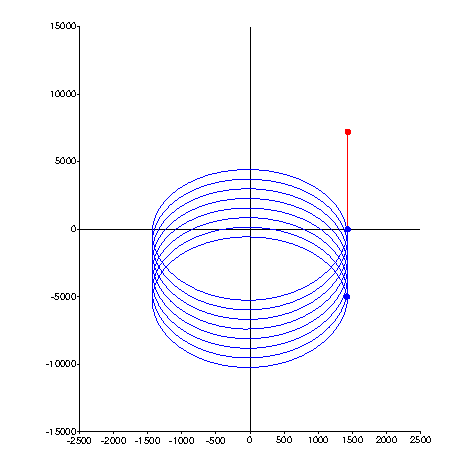
\includegraphics{trajectory.pdf}
\end{figure}

\end{document}
